\documentclass[11pt]{article}
\usepackage{graphicx}
\usepackage{subcaption}
\usepackage{wrapfig}
\title{Ubiquitous Genomics: Hackathon2}

\author{
  Maya Anand\\ mva2112@columbia.edu \and
  Cheyenne Parsley\\ cep2141@columbia.edu \and
  Robert Piccone\\ rap2186@columbia.edu \and
  Daniel Speyer\\ dls2192@columbia.edu}
\begin{document}
\maketitle
\section*{Problem 1}
Number of 2D reads classified as failed: 258\\
Number of 2D reads classified as passed: 1082\\
\section*{Problem 2}
\begin{wrapfigure}{r}{2.5in}
  \vspace{-20pt}
  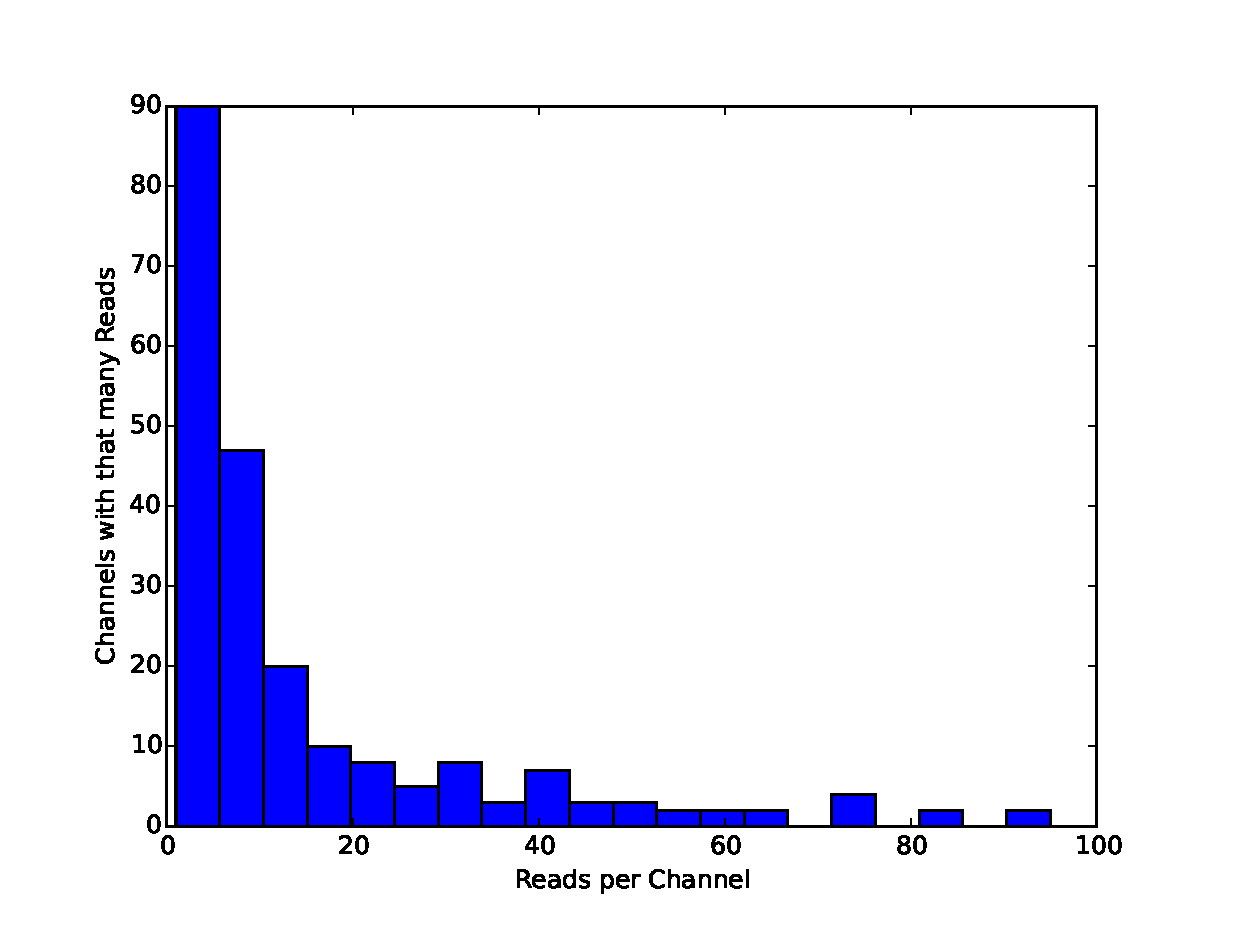
\includegraphics[width=2.5in]{part2hist}
  \vspace{-20pt}
\end{wrapfigure}
255 channels had at least one read, and 216 had at least five.  
This compares with 412 ``active'' channels during initialization, and 618 immediately after loading fuel

The average channel had 9.9 reads. 
Channel 53 had 67 reads, which was the most.

Just for fun, here's a histogram of reads per channel\\
\newpage
\section*{Problem 3}
\subsection*{Failed Reads}

        The following plots show the length distribution of 2D and 1D reads for fails.
       
        \begin{tabular}{cc}
          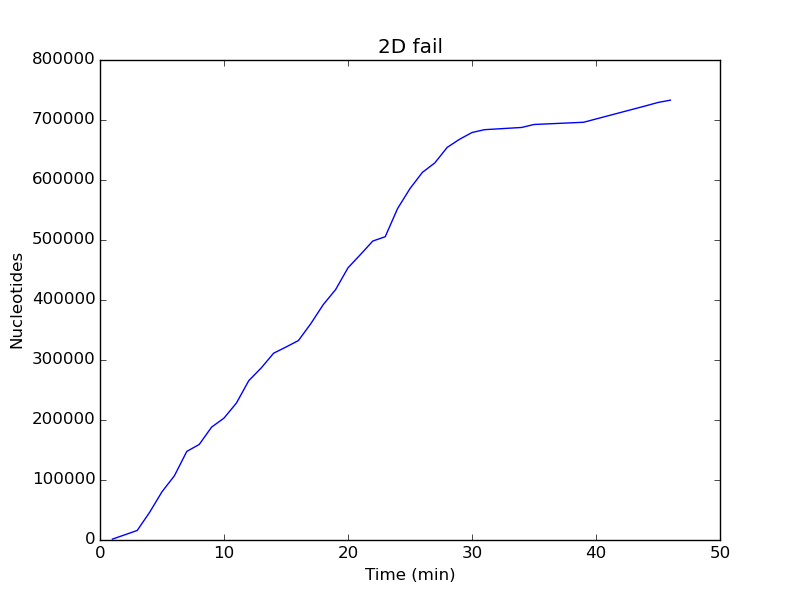
\includegraphics[width=.48\textwidth]{failcum2D}
          &
          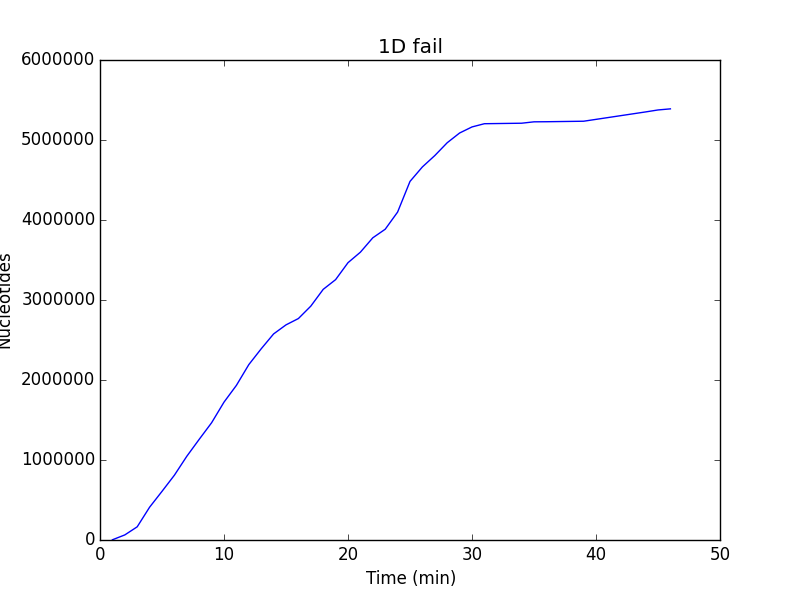
\includegraphics[width=.48\textwidth]{failcum1D}
          \\
          2D Reads
          &
          1D Reads
        \end{tabular}

\subsection*{Passed Reads}

        The following plots show the length distribution of 2D and 1D reads for passes.

        
        \begin{tabular}{cc}
          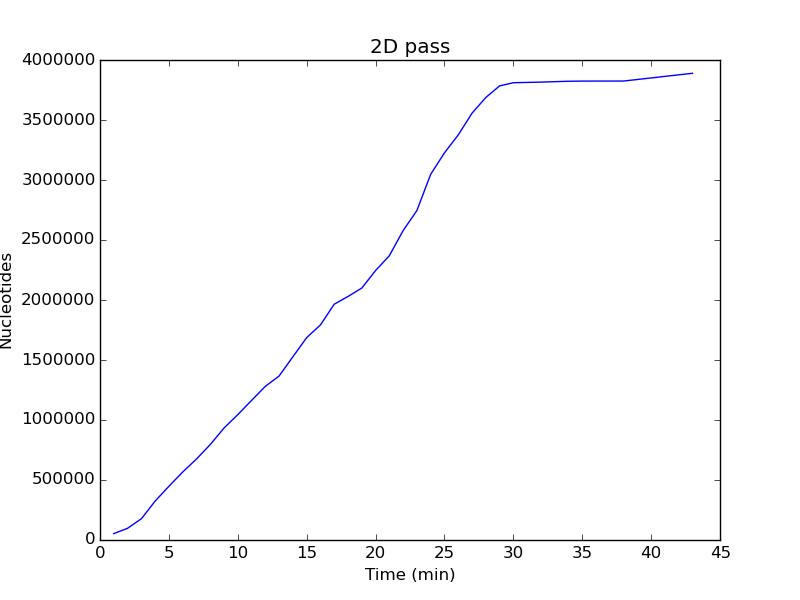
\includegraphics[width=.48\textwidth]{passcum2D}
          &
          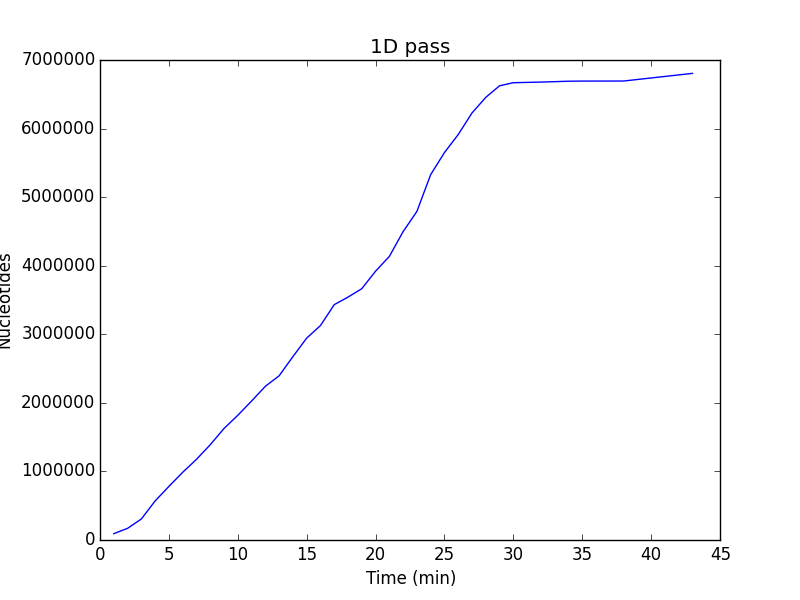
\includegraphics[width=.48\textwidth]{passcum1D}
          \\
          2D Reads
          &
          1D Reads
        \end{tabular}
\newpage
\section*{Problem 4}
\subsection*{2D reads}

        The following histograms show the length distribution of 2D reads for passes and fails.

        
        \begin{tabular}{cc}
          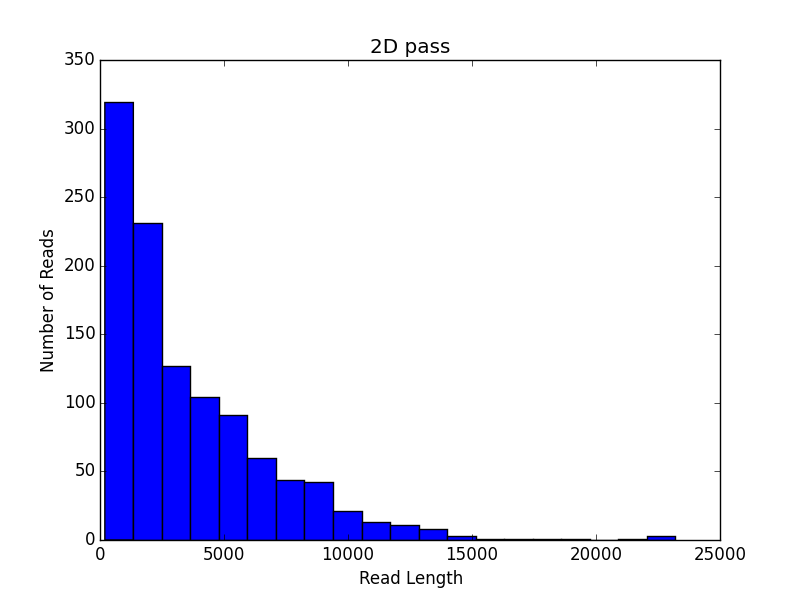
\includegraphics[width=.48\textwidth]{2Dpasses}
          &
          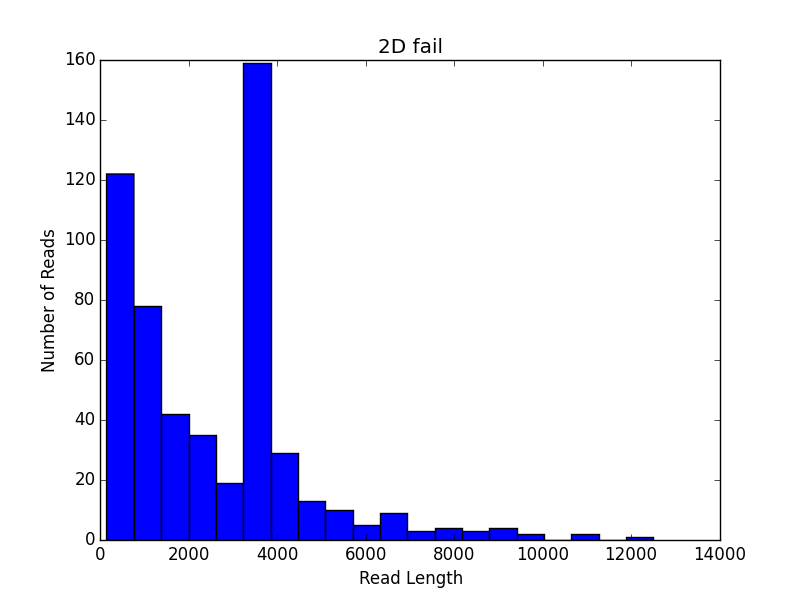
\includegraphics[width=.48\textwidth]{2Dfailures}
          \\
          Passed Reads
          &
          Failed Reads
        \end{tabular}
\section*{Problem 5}

LONGEST PASSED 2D READ\\
From file: MINION02\_Hackathon2\_group4\_TeamAWESOME\_4029\_1\_ch9\_file8\_strand.fast5\\
Number of nucleotides: 23196\\

LONGEST FAILED 2D READ\\
From file: MINION02\_Hackathon2\_group4\_TeamAWESOME\_4029\_1\_ch360\_file3\_strand.fast5\\
Number of nucleotides: 13419\\
\section*{Problem 6}
Total \# of aligned reads: 851\\
Total \# of unaligned reads: 231\\
\\
Total \# of reads: 1082\\
\section*{Problem 7}
As with hackathon1, only some of the reads could be aligned and of those only portions of them.  The usual concerns about selection bias apply.  Furthermore, finding the reference sequence for alignments to the complement strand proved difficult, so we offer here only the reads which aligned to the template strand.

This table shows count of nucleotides from those alignments.  Rows indicate the nucleotide in the reference genome, columns in the read returned by MinION.


\begin{tabular}{r||r|r|r|r|r}
  & A & C & G & T & -\\ \hline
\hline
A & 170885 & 3697 & 4060 & 1611 & 11374\\ 
\hline
C & 2084 & 116750 & 2586 & 2262 & 6074\\ 
\hline
G & 2515 & 2554 & 114255 & 1837 & 6446\\ 
\hline
T & 1741 & 3952 & 3316 & 171694 & 10925\\ 
\hline
- & 10330 & 11696 & 12358 & 9871 & 0\\ 
\end{tabular}
\section*{Problem 8}
To reduce the number of errors in the reads, we could have tried several methods:

First, we could replicate the DNA with PCR using random primers to have more copies of
fewer fragments. By sequencing multiple fragments of the same sequence we could have some redundancy and 
use that to cross-check our data.

Next, we could look at the quality scores and only pay attention to high ones.
This could lead to throwing out poor data, and improving the overall accuracy
of the reads. Though this sounds like a solid strategy in theory, it should be
noted that in the last hackathon, we found that the quality scores were not
very good. Also, if there were certain sequences that are specifically difficult to sequence
for whatever reason, this method would not include them, introducing selection bias.

Finally, we could improve accuracy by only believing polymorphisms that are known 
to be in $>$1\% of the population. Otherwise, we must believe it is a sequencing error, and
not a variation. 
\end{document}
